\subsection{Sidelobes}

\paragraph{Description:}
The angular response of an optical system (given by its point spread function $P(\theta, \phi)$) consists of a \emph{main beam} and \emph{sidelobes}. The main beam is the region to which the system is the most sensitive to light. Sidelobes are directions from where, though not in the main beam, still some light can be detected at the focal plane usually attenuated (by several 10s of dBs) below the main beam intensity, see Figure~\ref{fig:cartoonSidelobe}.

Sidelobes can be classified in near and far, depending on their angular position relative to the main beam.

\begin{figure}[h]
\label{fig:cartoonSidelobe}
\centering
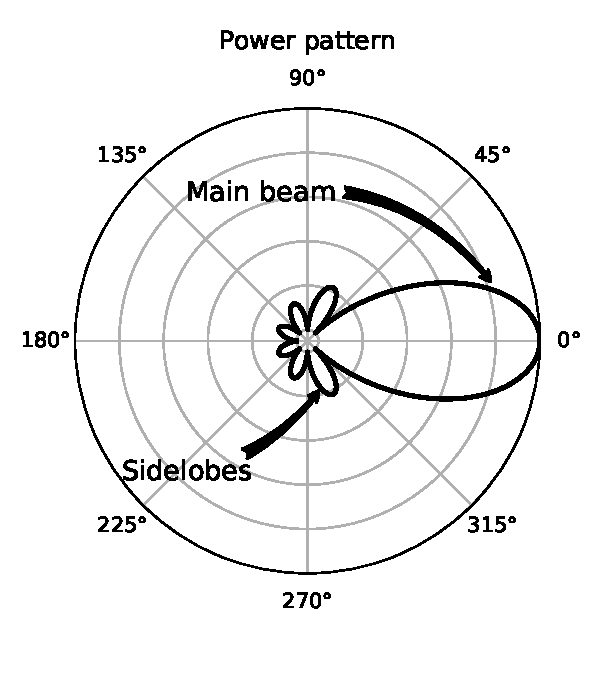
\includegraphics[width=0.45\textwidth]{sidelobeCartoon.pdf}
\caption{Cartoon representation of $P(\theta)$. Note that the angular response peaks around 0 degrees and sidelobes extend even to the back of the system.}
\end{figure}


\begin{description}
\item[Near sidelobes] are sidelobes that are close ($\frac{\lambda}{D}$ - 1FoV) to the main beam. They can be generated by diffraction (ringing in the Airy function), ghosting (reflections between optical components), stray reflections (reflections on the baffling structures) and scattering in optical components to name a few. Their intensity is $O(10\times)$ lower than the main beam or weaker.

\item[Far sidelobes] occur from 1 FoV to 180 degrees from the main beam. They are typically attenuated more than 20 dBs, are hard to measure and require detailed modeling or experiments to be identified and understood. Sources of far sidelobes are: reflections/diffraction over the physical structure of the telescope and scattering over optical components. 
\end{description}

The physical mechanism that generates a sidelobe can correspond in general to a combination of simpler mechanisms, some of which are listed below: 

\begin{description}
\item[Diffraction]

Sharp edge diffraction can cause sidelobes. In a perfect circular aperture case, diffraction around an aperture with uniform illumination will cause a sidelobe at the second maximum of the function $2J_1(x)/x$ which is 17.83dB below the peak.

\item[Ghosting]

Reflections inside a refractive camera can cause the phenomenon known as ghosting. Light coming through the camera gets reflected off an optical component and this reflection is re-imaged, creating a false image at the focal plane. Optical elements that can contribute to ghosting are: a reflective focal plane composed of metalized feedhorns/reflective lenslets, partially reflective lenses or filters, and a partially blackened optics tube interior.

\item[Stray Reflections]

Off-axis light can be reflected by surfaces that are not perfectly black in the baffling structure of a refractive system, creating a sidelobe. This sidelobe, in the case of a large aperture telescope can interact with the telescope support structure generating a complex pattern.

\item[Scattering in optical components]

Scattering refers to any reemission of light passing through a material. The angular dependence of this reemission depends on the details of the properties of the material but in general is not necessarily specular.

\item[Panel Gap Diffraction]
Primary and secondary mirrors are commonly built from individual panels. The gaps between these panels can interact with the incident light forming a complicated diffraction pattern that creates sidelobes. These sidelobes can extend over several degrees and can be polarized \cite{fluxa_rojas_far_2016}.

\item[Ruze Scattering]
Gaussian surface errors on reflector elements can also cause distortions to the main beam. For a detailed description of this effect see Section~\ref{sec:ruze}.

\end{description}

\paragraph{Plan to model and/or measure:}

A variety of techniques exist for modeling large structures. Vector Physical Optics models (including Physical Theory of Diffraction) give very detailed sidelobe patterns, though computation time is generally long. For high frequencies (above 150GHz), solving a ~10 meter physical structure can take months with modern (16 cores) computers. For this reason, faster techniques are generally used in the design stages, where rapid prototyping is a priority. The design of the Simons Observatory uses vector Physical Optics for the modeling of the main beam and near sidelobes, while the far sidelobe pattern is modeled using a ray tracing model with parameters informed from former measurements of the camera beam of other CMB experiments. This approach gives a fast first order approximation of the far sidelobe pattern of the optical system. Computation times (for a 4 core desktop) in this case take anywhere from minutes to hours depending on the level of sampling necessary.

Near sidelobes can be characterized by observing point sources, and planets are typically used. Far sidelobes can be characterized using moon/sun centric maps. This technique has been used to describe the sidelobe pattern of the Atacama Cosmology Telescope (Gallardo 2018 in prep.). Other metrics like near field spillover can be measured in situ and used to inform a sidelobe model.

Sidelobes can cause serious issues, especially when they pick up the ground or bright sources like the sun. Proper baffling must be used and the scanning pattern must have sun avoidance built in. All of these are critical to the design, so this systematic has an SRF of 5.
\paragraph{Uncertainty/Range:}
For an off-axis system, the sidelobe intensity is expected to be below 50dB from the main beam \cite{lockman_stray_2002}. This is consistent with near field experiments at the Atacama Cosmology Telescope \cite{dunner_far_2012} and with the sidelobe level reported in \cite{naess_atacama_2014}.


\paragraph{Parametrization:} Metrics of sidelobe performance include: the sidelobe solid angle $\Omega_{sl}$ and the overall intensity below the main beam. Also, for polarimetry, a detailed map of polarization properties is important. Fiducial sidelobe templates informed by a combination of optical modeling for proposed designs and historical precendence can be also be generated and incorporated with the a scan strategy to understand the impact on the scientific goals of an experiment.

